\documentclass{ximera}

\input{../../preamble.tex}
\author{Bobby Ramsey}

\begin{document}
\begin{exercise}
	A ladybug is traveling along the curve $y=2\sqrt{4x+9}$.
	\begin{center}
		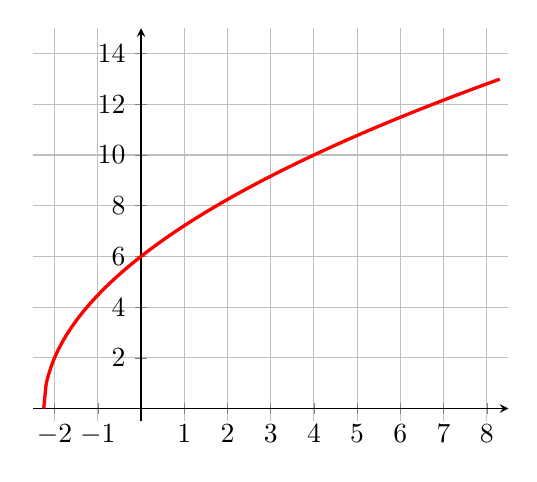
\begin{tikzpicture}
			\begin{axis}[
				xmin=-2.5, xmax=8.5, ymin=-0.5,ymax=15,    
				axis lines =middle, 
				every axis y label/.style={at=(current axis.above origin),anchor=south},
				every axis x label/.style={at=(current axis.right of origin),anchor=west},
				xtick={-2,...,8}, ytick={0,2,...,14},
				grid=major, width=3in,
				]
				\addplot[color=red, very thick, smooth, samples=200,domain=-2.25:8.3]{2*(4*x+9)^(0.5)};
			\end{axis}
		\end{tikzpicture}
	\end{center}
	As the ladybug passes through the point $(4,10)$, its $x$-coordinate increases at a rate of $3$ units/sec.  How
	fast is the distance from the ladybug to the origin growing at this instant?

	\[ \text{The distance is growing at } \, \answer{\frac{36}{\sqrt{116}} \, \text{ units/sec} \]
\end{exercise}

\end{document}

